\documentclass[10pt]{article}
\usepackage[utf8]{inputenc}
\usepackage{geometry}
\usepackage{graphicx,graphics}
\usepackage{hyperref}
\usepackage{graphicx}
\usepackage{url}
\usepackage{float}
\usepackage{amsmath}
\usepackage{multicol}
\usepackage{amssymb}
\usepackage{multirow}
\usepackage{textcomp}
\usepackage{gensymb}
\usepackage{hhline}
\usepackage{array}
\usepackage{caption}
\usepackage[spanish, es-tabla]{babel}
\usepackage[center]{titlesec}
\usepackage[table,xcdraw]{xcolor}

\geometry{top=2cm, bottom=2cm, left=1.5cm, right=1.5cm}
\spanishdecimal{,}
\setlength{\parskip}{0mm}

\renewcommand{\arraystretch}{1.3}
\renewcommand{\thesection}{\large\Roman{section}}
\renewcommand{\thesubsection}{\large\Alph{subsection}}

\providecommand{\abs}[1]{\lvert#1\rvert}
\title{
    Estudio del Equilibrio Químico y la Constante de Equilibrio mediante laboratorios virtuales
}
\author{
    \normalsize{
        \emph{Andrés F. Valencia Fonseca}$^{1}$,
        \emph{Nicolás Aguilera García}$^{2}$
    } \\
    \normalsize{
        \emph{Departamento de Física, Universidad del Valle, Cali, Colombia}
    } \\
    \small{$^{1}$2125166, $^{2}$21273030}
}
\date{(\small 3 de junio de 2023)}

\begin{document}
\maketitle
\begin{abstract}
    En este informe de laboratorio, se llevó a cabo un estudio sobre la constante de equilibrio y su importancia en las reacciones químicas reversibles. Se utilizó el hecho de que la constante de equilibrio ($K_c$) se calcula utilizando las concentraciones de los reactivos y productos, elevadas a sus coeficientes estequiométricos. A partir de este concepto, se realizaron experimentos en un laboratorio virtual para investigar el comportamiento de las concentraciones en el equilibrio en función de diferentes valores de $K_c$. Se encontró que cuando $K_c < Q$, la reacción se desplaza hacia la formación de reactivos, mientras que si $K_c > Q$, se favorece la formación de productos. También se verificó la precisión de los cálculos de las concentraciones en el equilibrio para diferentes condiciones iniciales y valores de $K_c$. Estos resultados demostraron la utilidad de la constante de equilibrio para predecir el sentido en el que evoluciona una reacción reversible.
\end{abstract}

\begin{multicols*}{2}
    \section{\small INTRODUCCIÓN}
    Las reacciones químicas pueden ocurrir en diferentes direcciones. Algunas reacciones avanzan hacia la formación de productos, mientras que otras pueden revertirse, volviendo a los reactivos originales. En el caso de las reacciones reversibles, después de cierto tiempo, se alcanza un estado llamado equilibrio químico.

    El equilibrio químico se caracteriza por un estado en el que la velocidad de la reacción hacia adelante es igual a la velocidad de la reacción en sentido inverso. En este punto de equilibrio, tanto las concentraciones de los productos como las de los reactivos se mantienen constantes. Es importante destacar que el equilibrio no implica que la reacción se haya detenido, sino que ambas reacciones (hacia adelante y en sentido inverso) siguen ocurriendo simultáneamente \cite{giancoli}.

    La constante de equilibrio ($K_c$) se define como la relación de las concentraciones de los productos elevadas a sus coeficientes estequiométricos, dividida por las concentraciones de los reactivos elevadas a sus coeficientes estequiométricos. Para una reacción química balanceada, la expresión de $K_c$ se establece como:

    \begin{equation}
        K_c = \frac{[C]^c[D]^d}{[A]^a[B]^b}
        \label{eq:kc}
    \end{equation}

    Donde $A$, $B$, $C$ y $D$ representan las concentraciones molares de los reactivos y productos respectivamente, y $a$, $b$, $c$ y $d$ son los coeficientes estequiométricos de la ecuación balanceada.

    El valor de $K_c$ es específico para una reacción química en particular y se determina experimentalmente a una temperatura específica. Es importante tener en cuenta que $K_c$ no se ve afectado por las concentraciones iniciales de los reactivos, sino que solo depende de la temperatura de la reacción. Si el cálculo de $K_c$ se realiza antes de alcanzar el equilibrio se denota como coeficiente de reacción $Q$.

    El valor de $K_c$ proporciona información crucial sobre la dirección en la que se favorece una reacción reversible. Si $K_c$ es mayor que 1, se favorece la formación de productos en el equilibrio, mientras que si $K_c$ es menor que 1, se favorece la formación de reactivos. Además, si $K_c$ es igual a 1, indica que las concentraciones de los productos y reactivos están en equilibrio.

    \section{\small METODOLOGÍA}
    En este informe de laboratorio, se llevó a cabo una práctica utilizando un laboratorio virtual para estudiar el equilibrio químico y la constante de equilibrio ($K_c$) en una reacción que involucra dos reactivos y dos productos, todos con un coeficiente estequiométrico igual a $1$.

    En primer lugar, se ajustaron las concentraciones de todas las especies químicas a un valor constante de $0.5 , \text{mol/L}$. A continuación, se varió la constante de equilibrio $K_c$, tomando los valores de $0.01$, $0.1$, $1$, $10$ y $100$. Para cada valor de $K_c$, se registraron las concentraciones de cada especie en el estado de equilibrio alcanzado.

    Posteriormente, se seleccionó una concentración inicial de $1 , \text{mol/L}$ para los reactivos y $0 , \text{mol/L}$ para los productos. Nuevamente, se varió la constante de equilibrio $K_c$, esta vez utilizando los valores de $0.01$, $0.05$, $0.1$, $0.5$, $1$, $5$, $10$, $50$ y $100$. Se analizó el comportamiento de las concentraciones en el equilibrio en función de los diferentes valores de $K_c$.

    En la siguiente etapa, se establecieron concentraciones iniciales de $1 , \text{mol/L}$ para los reactivos y $0 , \text{mol/L}$ para los productos, utilizando un valor específico de $K_c = 5$. Se realizó el cálculo de las concentraciones en el equilibrio para cada especie química para posteriormente verificarlas con los valores obtenidos en el laboratorio virtual.

    Finalmente, se repitió el procedimiento anterior, pero en esta ocasión se estableció una concentración inicial de $1 , \text{mol/L}$ tanto para los productos como para los reactivos.

    Cabe destacar que todas las etapas de la práctica se llevaron a cabo en el laboratorio virtual.

    \section{\small ANÁLISIS Y RESULTADOS}
        Empezando con la determinación del cociente de reacción $Q$ para el caso en el que las concentraciones iniciales de los reactivos y productos son iguales a $0.5 , \text{mol/L}$, se obtuvieron los siguientes resultados. Se obtuvo que el valor de $Q$ está dado por:

        \begin{equation}
            Q = \frac{[C]^c[D]^d}{[A]^a[B]^b} = \frac{[0.5]^1[0.5]^1}{[0.5]^1[0.5]^1} = 1
        \end{equation}

        Ahora bien, si se realizan variaciones en el valor de $K_c$ mientras se mantiene la concentración inicial de los reactivos y productos en $0.5 , \text{mol/L}$ (que también es el valor de $Q$), se obtienen los siguientes resultados:

        \begin{itemize}
            \item $K_c < Q$:
            
                Cuando ocurre que la relación entre $K_c$ y $Q$ es tal que $K_c < Q$, la reacción tenderá a la producción de reactivos, es decir, la reacción se moverá hacia la izquierda $A + B \rightleftharpoons C + D$. Esto se logró observar en todos los experimentos para condiciones de $K_c < Q$, las cuales fueron $K_c = 0.01$ y $K_c = 0.1$.

                \begin{figure}[H]
                    \centering
                    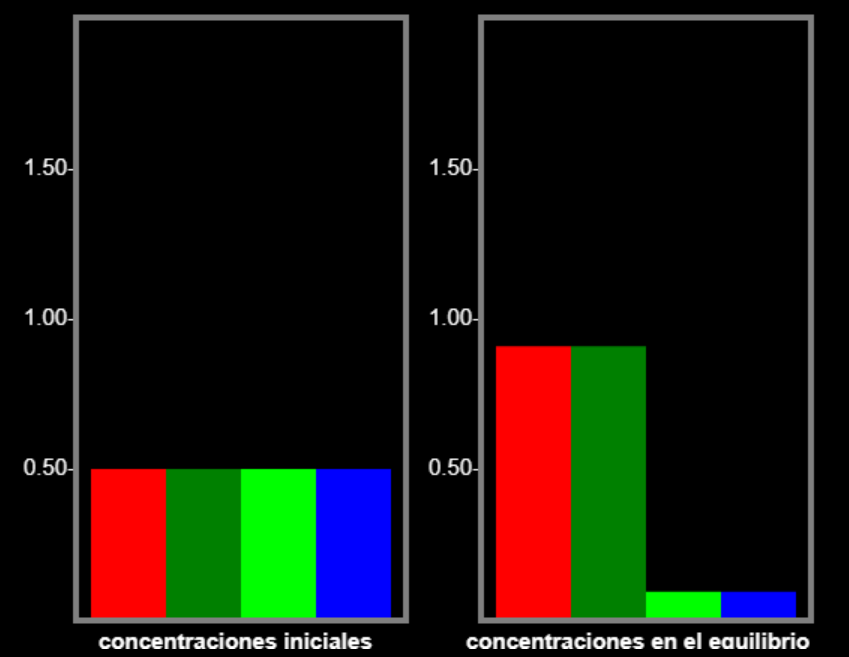
\includegraphics[width=0.35\textwidth]{img/lab001.png}
                    \caption{Concentraciones de las especies químicas en el equilibrio para $K_c = 0.01$}
                \end{figure}

                \begin{figure}[H]
                    \centering
                    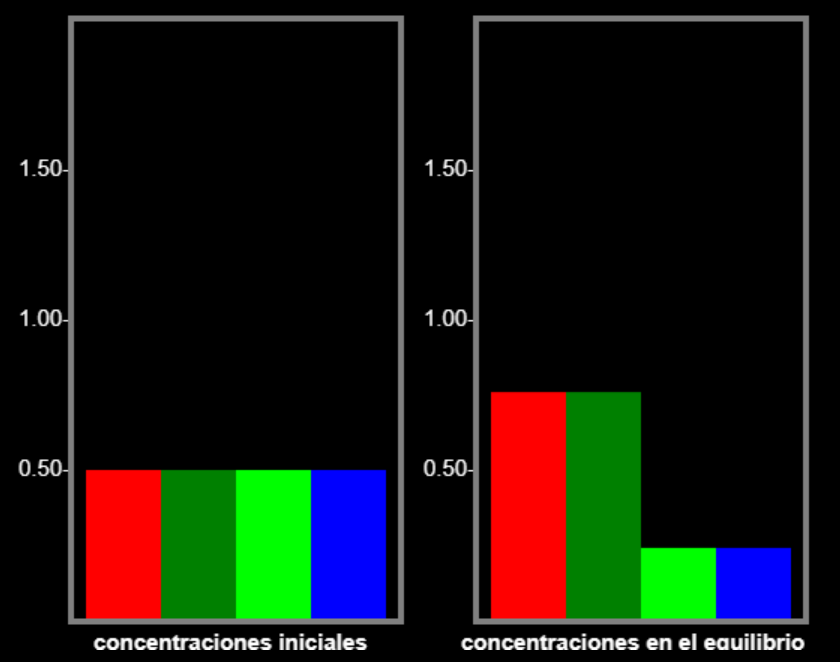
\includegraphics[width=0.35\textwidth]{img/lab01.png}
                    \caption{Concentraciones de las especies químicas en el equilibrio para $K_c = 0.1$}
                \end{figure}

            \item $K_c = Q$:

                Cuando ocurre que la relación entre $K_c$ y $Q$ es tal que $K_c = Q$, la reacción se encuentra en equilibrio, es decir, la reacción se encuentra en un estado en el que la velocidad de reacción de los reactivos hacia los productos es igual a la velocidad de reacción de los productos hacia los reactivos. Esto se logró observar en el experimento para condiciones de $K_c = Q$, la cual fue $K_c = 1$.

                \begin{figure}[H]
                    \centering
                    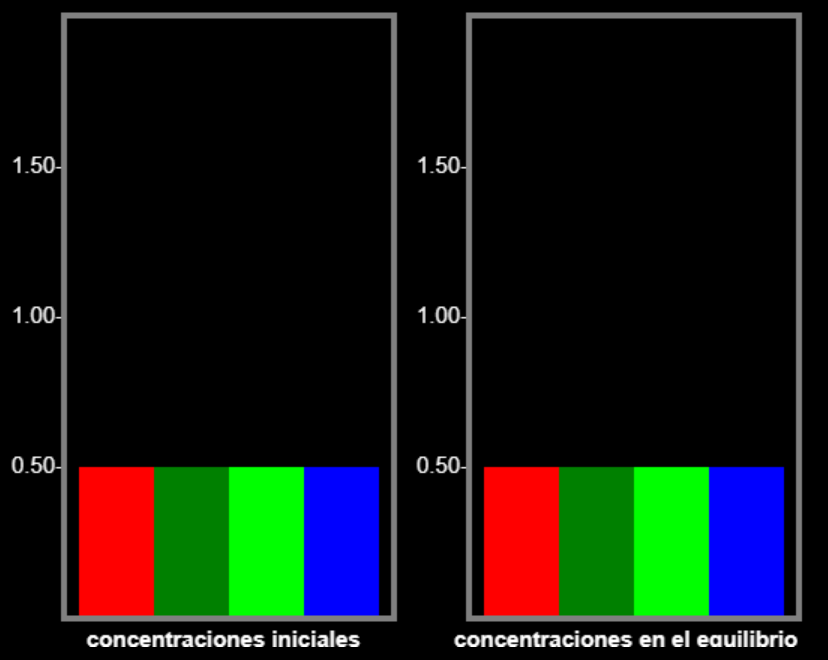
\includegraphics[width=0.35\textwidth]{img/lab1.png}
                    \caption{Concentraciones de las especies químicas en el equilibrio para $K_c = 1$}
                \end{figure}

            \item $K_c > Q$:

                Ahora, si ocurre que la relación entre $K_c$ y $Q$ es tal que $K_c > Q$, la reacción tenderá a la producción de productos, es decir, la reacción se moverá hacia la derecha $A + B \rightleftharpoons C + D$. Esto se logró observar en todos los experimentos para condiciones de $K_c > Q$, las cuales fueron $K_c = 10$ y $K_c = 100$.

                \begin{figure}[H]
                    \centering
                    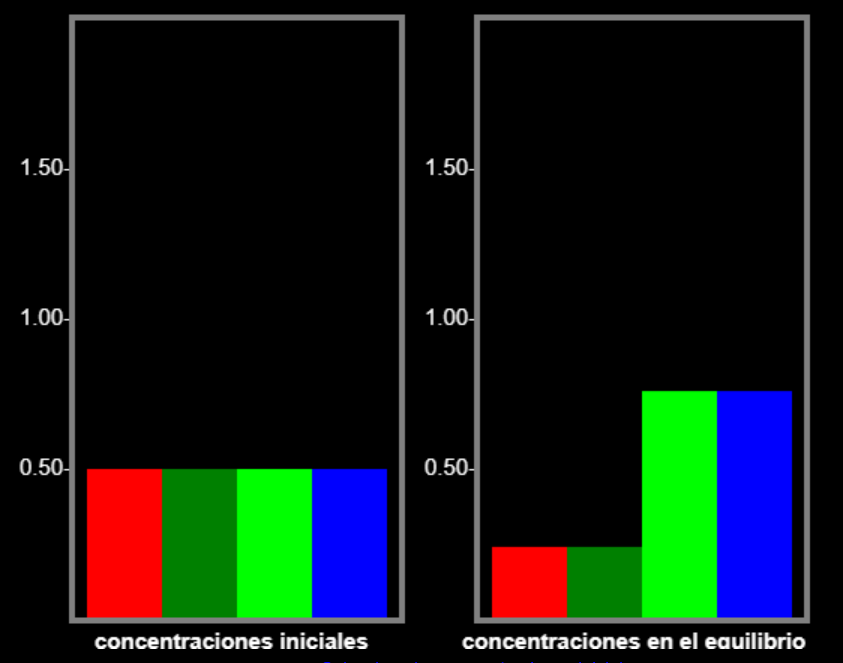
\includegraphics[width=0.35\textwidth]{img/lab10.png}
                    \caption{Concentraciones de las especies químicas en el equilibrio para $K_c = 10$}
                \end{figure}

                \begin{figure}[H]
                    \centering
                    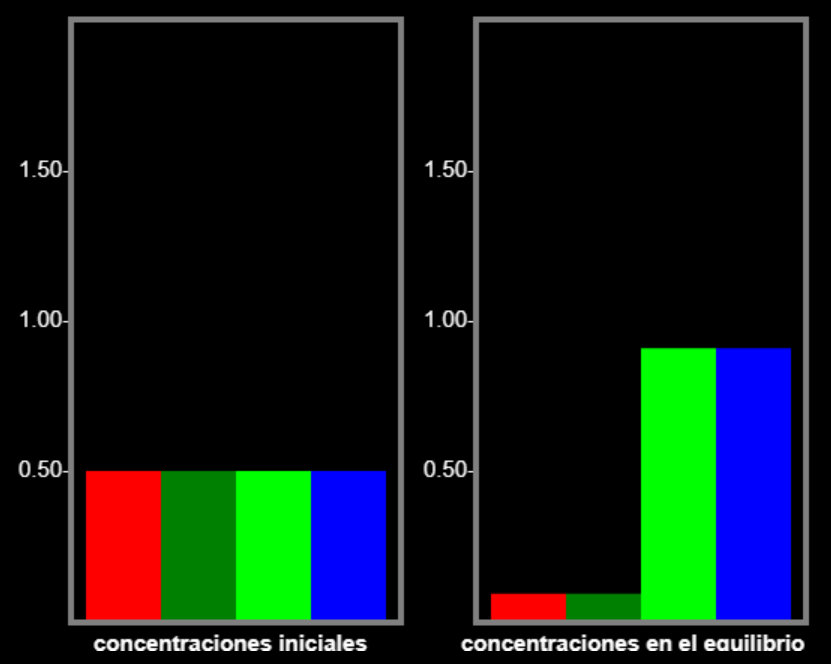
\includegraphics[width=0.35\textwidth]{img/lab100.png}
                    \caption{Concentraciones de las especies químicas en el equilibrio para $K_c = 100$}
                \end{figure}
        \end{itemize}

        Ahora bien, si se realizan variaciones en el valor de $K_c$ mientras se mantiene la concentración inicial de los reactivos en $1 , \text{mol/L}$ y la concentración inicial de los productos en $0 , \text{mol/L}$, se obtienen los siguientes resultados:

        \begin{figure}[H]
            \centering
            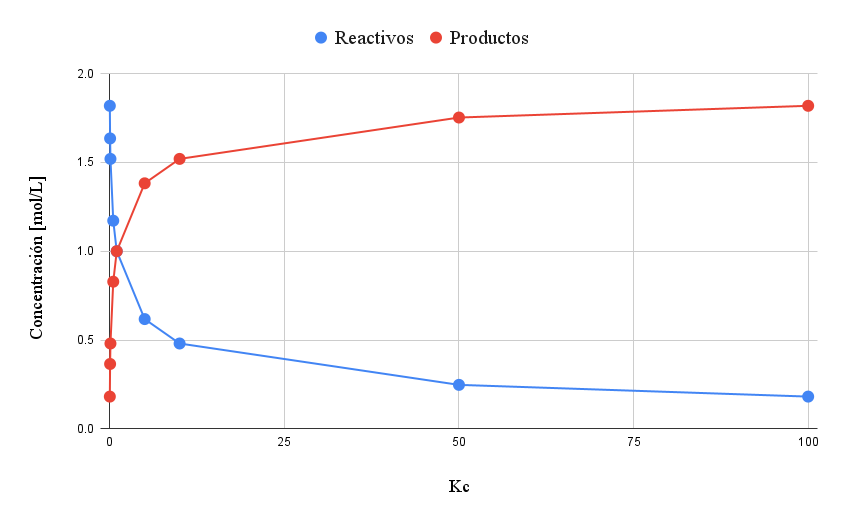
\includegraphics[width=0.48\textwidth]{img/chart.png}
            \caption{Comportamiento de las concentraciones de las especies químicas en el equilibrio en función del valor de $K_c$}
        \end{figure}

        En esta figura, es claro que a medida que el valor de $K_c$ aumenta, las concentraciones de los productos en el equilibrio también aumentan, mientras que las concentraciones de los reactivos disminuyen. Esto se debe a que a medida que el valor de $K_c$ aumenta, la reacción se mueve hacia la derecha $A + B \rightleftharpoons C + D$, lo que produce un aumento en las concentraciones de los productos y una disminución en las concentraciones de los reactivos.

        Finalmente, se determinó mediante la ecuación de equilibrio la concentración de las especies químicas en el equilibrio para el caso en el que las concentraciones iniciales de los reactivos son $1 , \text{mol/L}$ y para los productos son $0 , \text{mol/L}$, con una constante de equilibrio $K_c = 5$.

        \begin{equation}
            \begin{split}
                K_c &= \frac{[C]^c[D]^d}{[A]^a[B]^b} \\
                5 &= \frac{[C]^1[D]^1}{[A]^1[B]^1}
            \end{split}
        \end{equation}

        Si se plantea que $[A] = [B] = x$ y $[C] = [D] = y$, donde por las concentraciones iniciales se tiene que cumplir que $x + y = 1$, entonces se obtiene que:

        \begin{equation}
            \begin{split}
                5 &= \frac{y^2}{x^2} \\
                5 \cdot x^2 &= y^2 \\
                5 \cdot (1 - y)^2 &= y^2
            \end{split}
        \end{equation}

        Resolviendo la ecuación cuadrática, se obtiene que $y = 0.6909$ y $x = 0.3091$, lo que indica que las concentraciones de los reactivos en el equilibrio son $0.3091 , \text{mol/L}$ y las concentraciones de los productos en el equilibrio son $0.6909 , \text{mol/L}$. Lo cual es consistente con los resultados obtenidos en el laboratorio virtual.

        El mismo procedimiento es realizado para el caso en el que las concentraciones iniciales de los reactivos y los productos son de $1 , \text{mol/L}$, con una constante de equilibrio $K_c = 5$. Donde se obtiene que las concentraciones de los reactivos en el equilibrio son $0.618 , \text{mol/L}$ y las concentraciones de los productos en el equilibrio son $0.1382 , \text{mol/L}$. Lo cual es consistente con los resultados obtenidos en el laboratorio virtual.

    \section{\small CONCLUSIONES}
        Durante el laboratorio, se investigó el significado de la constante de equilibrio ($K_c$) y se realizaron experimentos para determinar cómo se desplaza la reacción hacia la formación de productos o reactivos. Se observó que cuando $K_c < Q$, la reacción se desplaza hacia la formación de reactivos, mientras que si $K_c > Q$, se favorece la formación de productos. Además, se pudieron calcular y verificar experimentalmente las concentraciones en el equilibrio para diferentes valores de $K_c$, a partir de las concentraciones iniciales de las especies químicas, lo que demuestra la utilidad de esta constante para predecir el comportamiento de las reacciones reversibles.

    \nocite{giancoli}
    \nocite{montiel2015física}

    \bibliographystyle{elsarticle-num}
    \bibliography{bib}
\end{multicols*}
\end{document}